% Gemini theme
% https://github.com/anishathalye/gemini

\documentclass[final]{beamer}

% ====================
% Packages
% ====================

\usepackage[T1]{fontenc}
\usepackage{lmodern}
\usepackage[size=custom,width=120,height=106.68,scale=1.5]{beamerposter}
\usetheme{gemini}
\usecolortheme{gemini}
\usepackage{graphicx}
\usepackage{booktabs}
\usepackage{tikz}
\usepackage{pgfplots}
\pgfplotsset{compat=1.14}
\usepackage{anyfontsize}
\usepackage{siunitx}
\usepackage{multicol}
\usepackage{physics}
\usepackage{bm}
\AtBeginDocument{\RenewCommandCopy\qty\SI}

% ====================
% Lengths
% ====================

% If you have N columns, choose \sepwidth and \colwidth such that
% (N+1)*\sepwidth + N*\colwidth = \paperwidth
\newlength{\sepwidth}
\newlength{\colwidth}
\setlength{\sepwidth}{0.025\paperwidth}
\setlength{\colwidth}{0.3\paperwidth} 

\newcommand{\separatorcolumn}{\begin{column}{\sepwidth}\end{column}}

% ====================
% Title
% ====================

% \title{MIDSX: A Monte Carlo Interaction and Dosimetry Simulation of X-rays}
% \title{\Large{MIDSX: A Monte Carlo Interaction and Dosimetry Simulation of X-rays}}
\title{\fontsize{80pt}{16pt}\selectfont MIDSX: A Monte Carlo Interaction and Dosimetry Simulation of X-rays}



\author{John Meneghini}

\institute[shortinst]{Department of Physics, Saint Vincent College, Latrobe, PA 15650}

% ====================
% Footer (optional)
% ====================

% \footercontent{
%   \href{https://www.example.com}{https://www.example.com} \hfill
%   ABC Conference 2025, New York --- XYZ-1234 \hfill
%   \href{mailto:alyssa.p.hacker@example.com}{alyssa.p.hacker@example.com}}
% (can be left out to remove footer)

% ====================
% Logo (optional)
% ====================

% use this to include logos on the left and/or right side of the header:
% \logoright{\includegraphics[height=7cm]{logo1.pdf}}
\logoleft{
\includegraphics[height=7cm]{svc_logo.pdf}}

\newcommand\zz[2][\colwidth]{\resizebox{\colwidth}{!}{\input{"#2.pgf"}}}


% ====================
% Body
% ====================

\begin{document}

\begin{frame}[t]
\begin{columns}[t]
\separatorcolumn

\begin{column}{\colwidth}

  \begin{block}{Introduction}
    \begin{itemize}
        \item CT imaging is essential but carries ionizing radiation risks.
        \item MC methods offer precise radiation estimation via photon transport simulations.
        \item Introducing MIDSX, an optimized open-source MC code for medical x-ray transport.
        \item MIDSX simplifies usage and is validated against benchmarks, proving its efficacy.
    \end{itemize}
    \vspace{-\baselineskip}
  \end{block}

  \begin{block}{Simulation Geometry}
    The geometry of a transport simulation consists of the following objects:
    \begin{itemize}
      \item A source object for photon generation.
      \item Voxel grids in NifTI files for object/body geometries and material info.
      \item Tallies for tracking photon trajectories and energy metrics.
      \item A computational domain for object containment and background material specification.
    \end{itemize}

    \begin{figure}
      \centering
      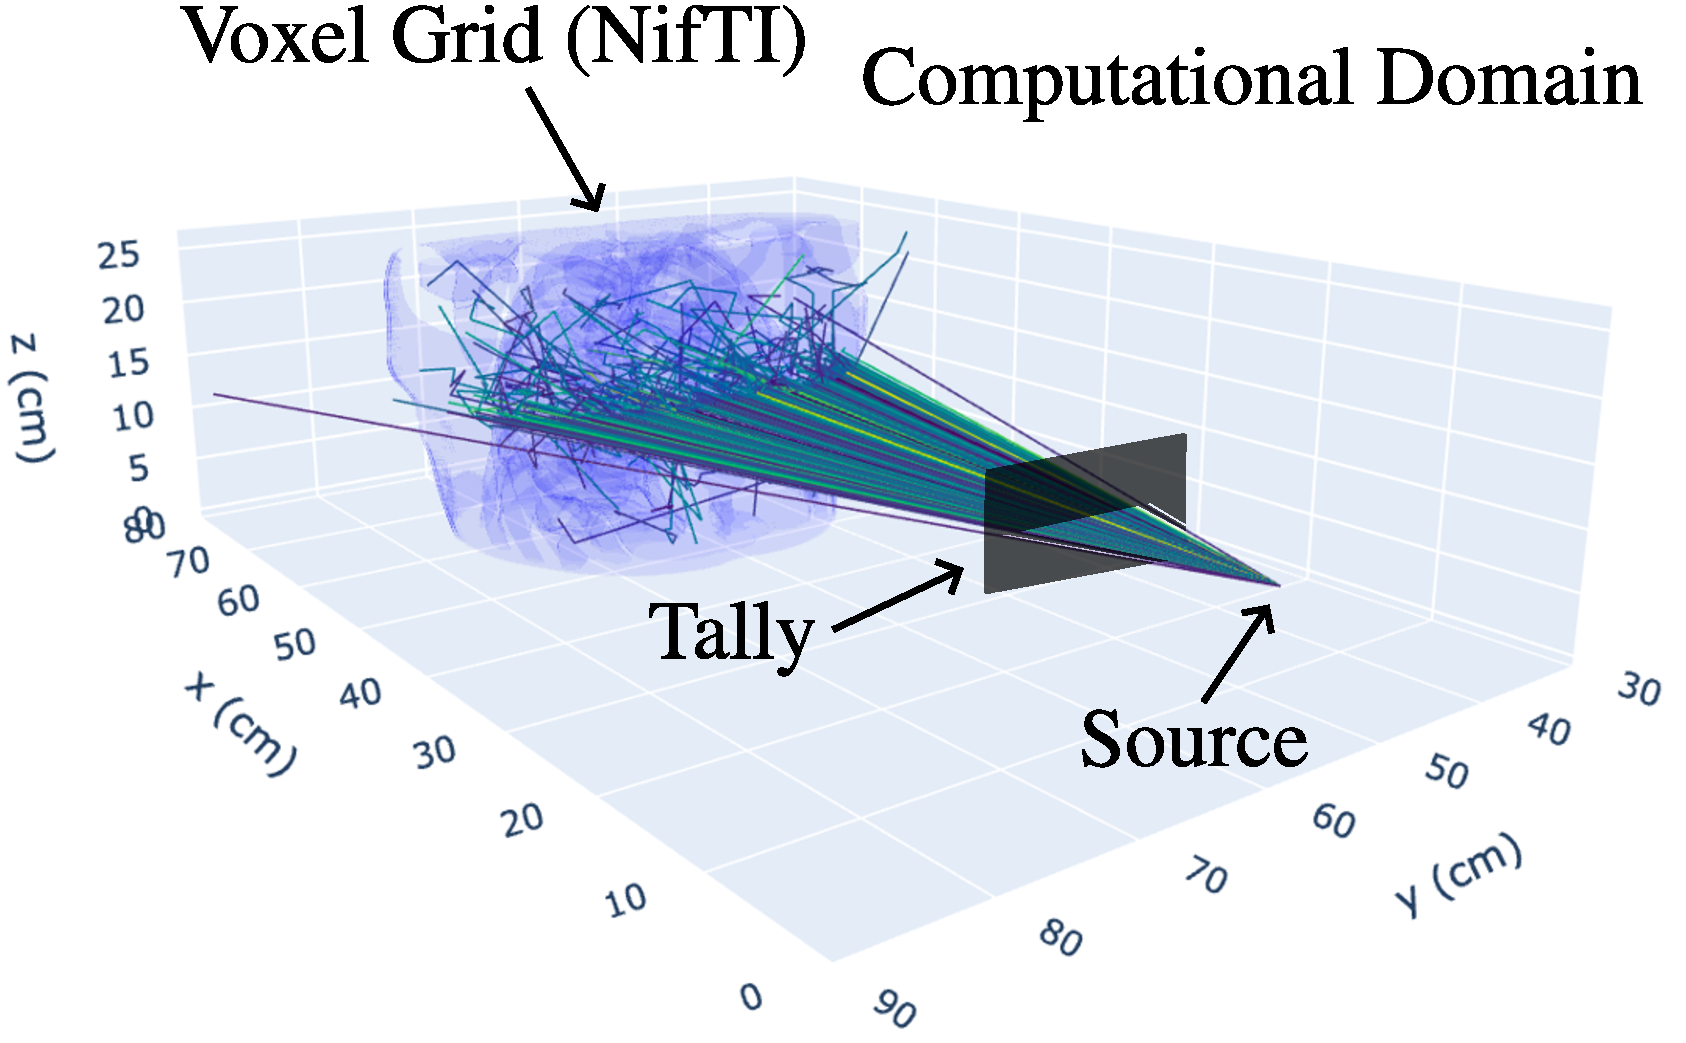
\includegraphics[width = 1\colwidth]{comp_domain.pdf}
      \caption{A typical transport geometry used in MIDSX.}
    \end{figure}
    \vspace{-\baselineskip}
  \end{block}

  \begin{block}{Transport Theory}

    \begin{figure}
      \centering
      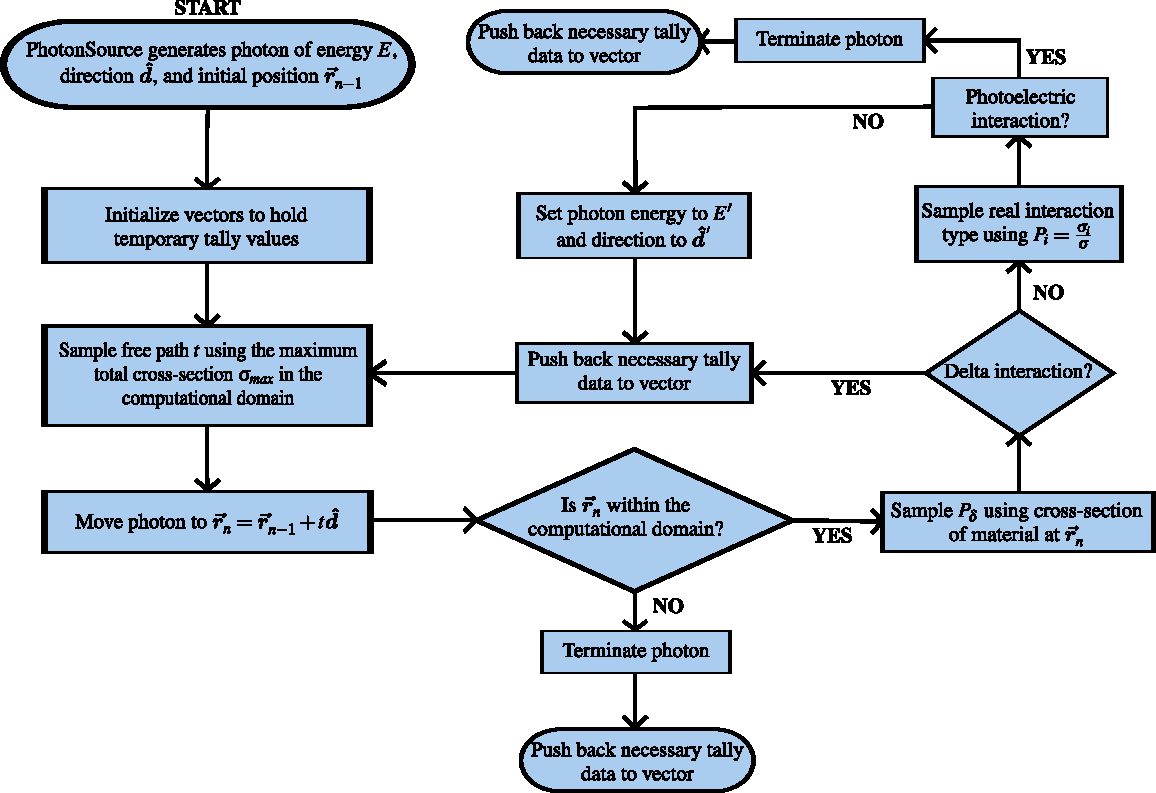
\includegraphics[width = 1.0\colwidth]{physics_engine_flow_chart.pdf}
      \caption{A flow chart showing the process behind a single photon step in the computational domain.}
    \end{figure}
    % \begin{itemize}
    %   \item As a photon take "steps" through a homogenous computational domain, its position after taking the $n$-th step is represented by the parametric ray equation:
    % \end{itemize}
    % \begin{equation} \label{eq:r_n}
    %     \va{r}_{\bm{n}} = \va{r}_{\bm{n-1}} + \vu{d}t,
    % \end{equation}
    % where $\va{r}_{\bm{n-1}}$ is the position before the $n$-th step, $\vu{d}$ is a unit vector in the direction of the step, and $t$ is the length of the $n$-th step.
    % \begin{itemize}
    %   \item For a photon of energy $E$ in material $M$, MIDSX randomly samples $t$ for use in Eq.~\ref{eq:r_n} from the following probability distribution function (PDF):
    % \end{itemize}
    % \begin{equation} \label{eq:pdf}
    %   p(t) = n\sigma \exp\left[-t(n\sigma)\right],
    % \end{equation}
    % where $n$ is the number density of $M$ and $\sigma = \sigma(E, M)$ is the microscopic cross-section of $M$ at $E$.
    % \begin{itemize}
    %   \item Using the inversion method for sampling a PDF on Eq.~\ref{eq:pdf}, random values of $t$ can be generated from
    % \end{itemize}
    % \begin{equation} \label{eq:t_inv}
    %   t = -\frac{1}{n\sigma} \ln \gamma, 
    % \end{equation}
    % where $\gamma$ is a uniformly distributed random number in the interval $[0, 1)$.

    % \begin{itemize}
    %   \item In order to generalize this to an inhomogeneous domain, MIDSX uses $\delta$ tracking \cite{vassiliev_monte_2017}.
    %   \item This effectively changes $\sigma \rightarrow \sigma_{\rm{max}}$ in Eq.~\ref{eq:pdf} and Eq.~\ref{eq:t_inv}, where $\sigma_{\rm{max}}$ is the maximum cross-section in the domain.
    %   \item In order to correct for the resulting systematic decrease in $t$, we implement $\delta$ interactions as an alternative to photon-matter interactions. The probability of which is given by 
    % \end{itemize}  

  \end{block}
\end{column}

\separatorcolumn

\begin{column}{\colwidth}

  % \begin{figure}
  %   \centering
  % 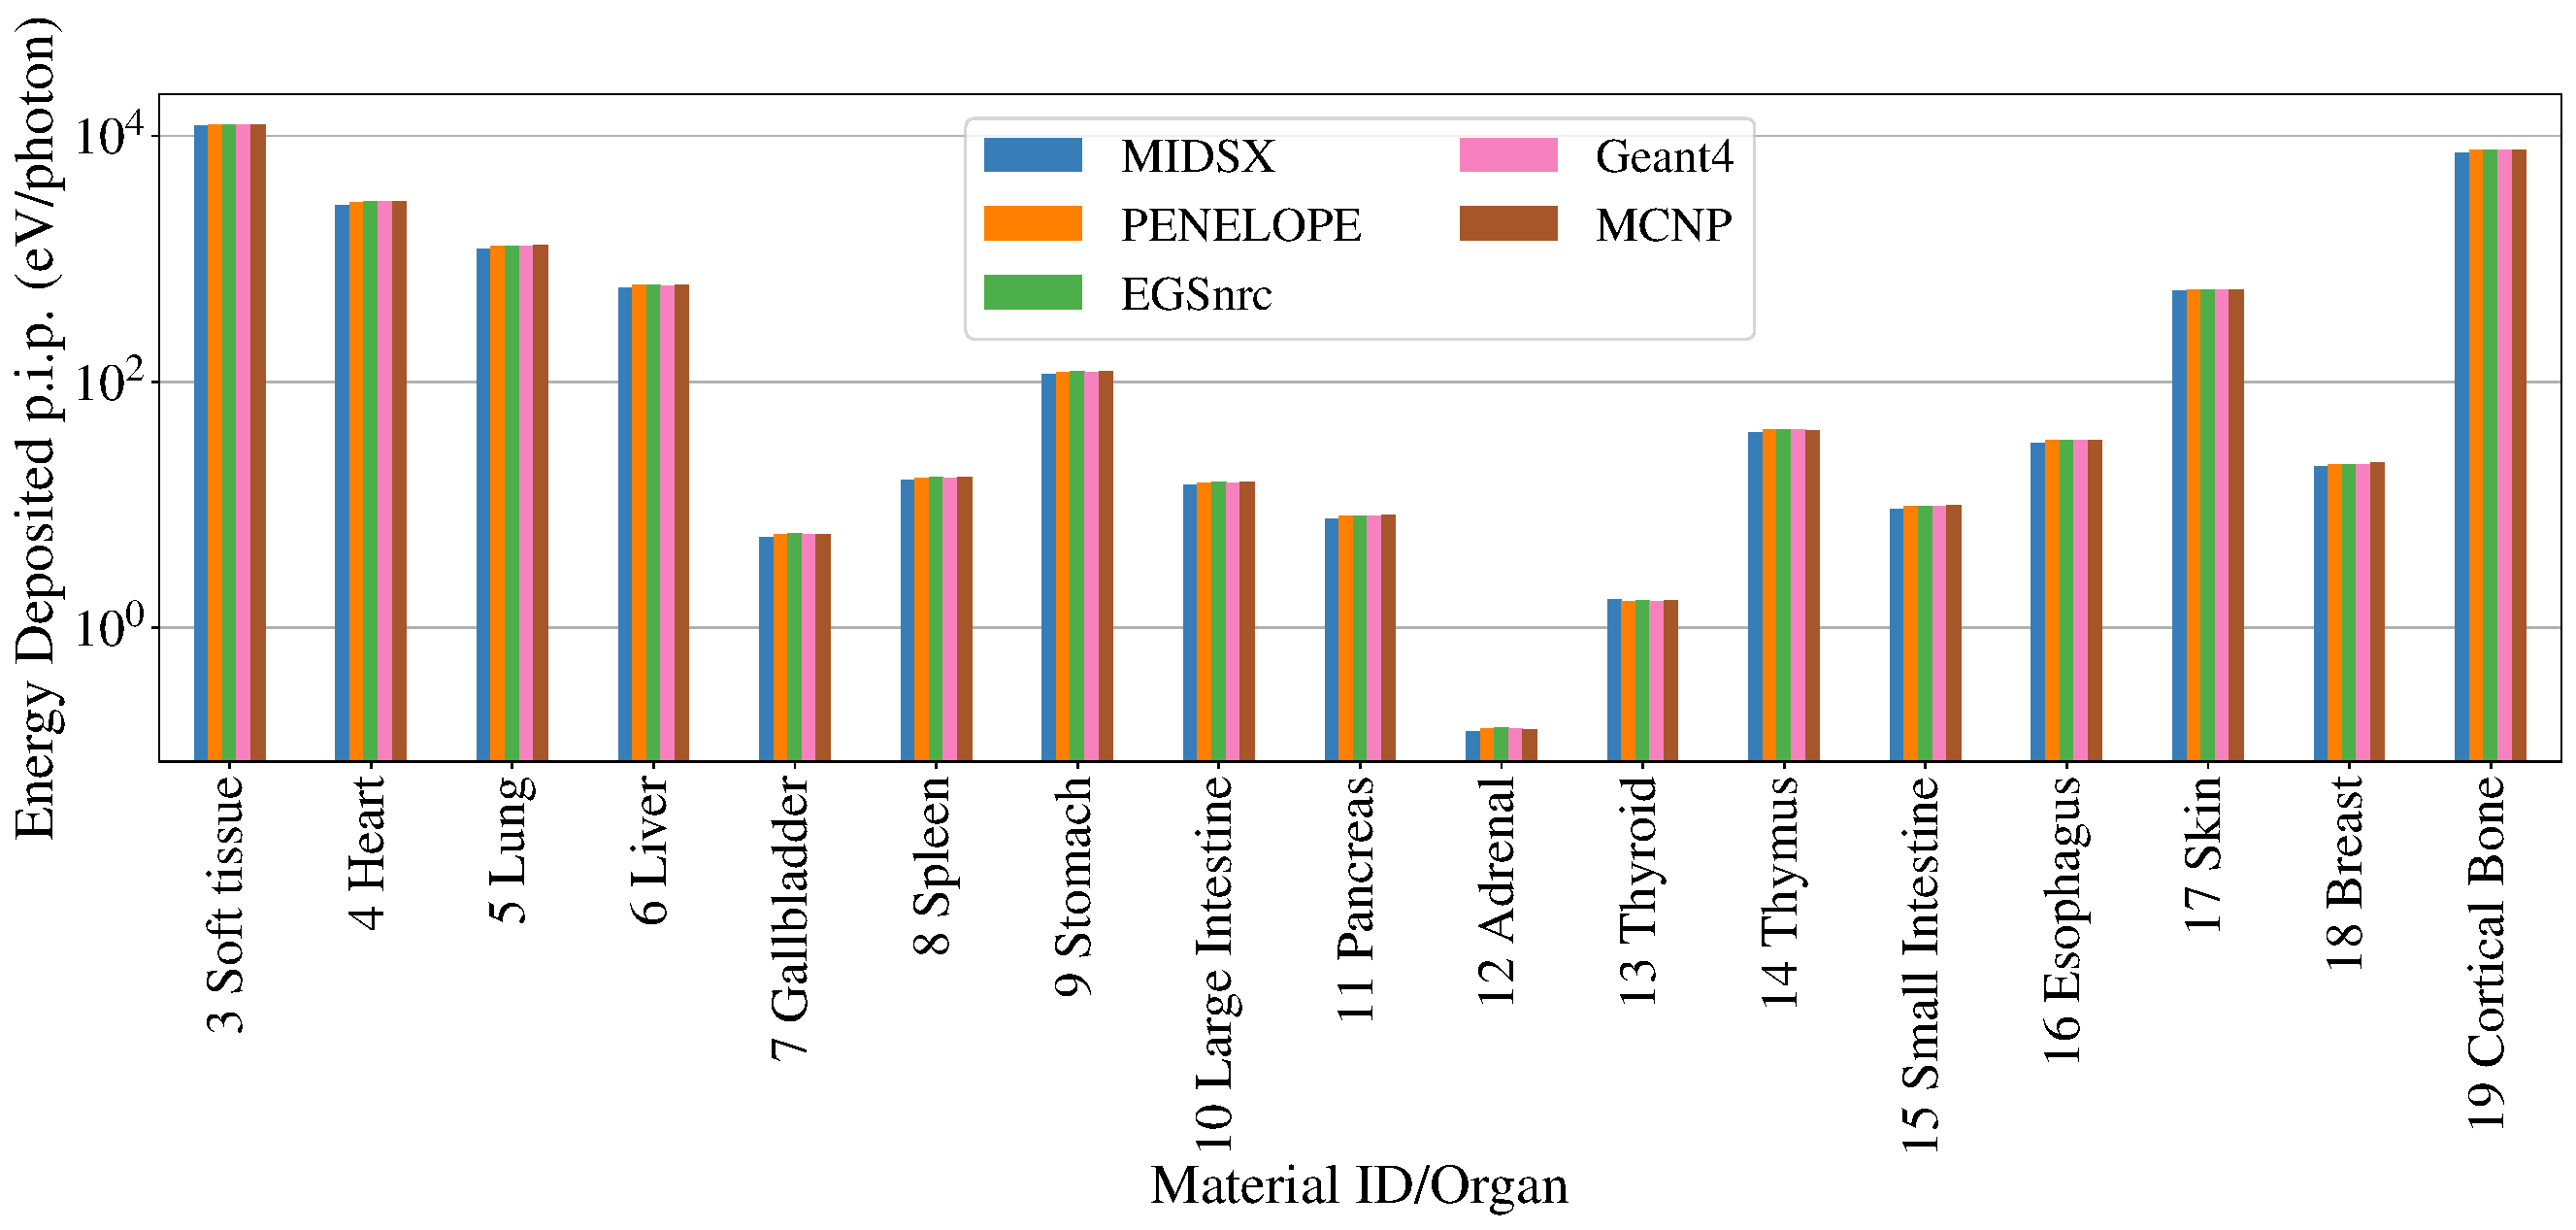
\includegraphics[width= 2\colwidth]{CT_120_0_big_font.pdf}
  % \caption{The energy deposited per initial photon (p.i.p.) (eV/photon) in the material IDs/organs composing a voxelized human phantom for the $0^\circ$, 120 kVp simulation as described by Case 5.}
  % \label{fig:CTGraph}
  % \end{figure}


  % \begin{equation}
  %   P_{\delta} = \frac{\sigma_{\text{max}}(E) - \sigma(E, M)}{\sigma_{\text{max}}(E)}.
  % \end{equation}

  % \begin{itemize}
  %   \item When a $\delta$ interaction occurs, nothing happens, and the next step is taken.
  % \end{itemize}  


  \begin{block}{Photon-Matter Interactions}
    If a $\delta$ interaction does not occur, then a real interaction is sampled. There are 3 fundamental possible photon-matter (real) interactions in the medical x-ray energy range that MIDSX implements:
    \vspace{-0.5\baselineskip}
    \begin{center}
      \textbf{Common Variables}
    \end{center}

    \begin{multicols}{2}
      \begin{center}
        $E$ - Energy of incoming photon\\
        $\theta_e$ - Angle of ejected electron\\
        \vspace{\baselineskip}
        \textbf{1. Photoelectric Effect}
      \begin{itemize}
        \item Photon interacts with electron of target atom, resulting in an electron being ejected with $E_e = E - U_i$ and the photon being absorbed.
      \end{itemize}
      \end{center}
      \vfill
      \begin{figure}
        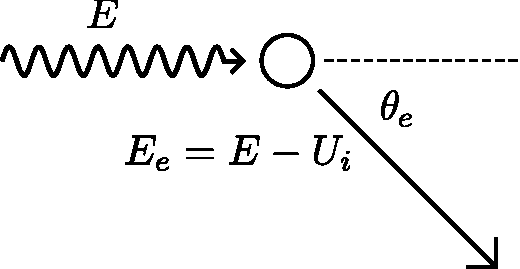
\includegraphics[width = 0.4\colwidth]{photoelectric_diagram.pdf}
        \caption{A diagram representing the photoelectric effect.}
      \end{figure}
      \columnbreak%
      \begin{center}
        $\theta$ - Angle of scattered photon \\
        $U_i$ - Binding energy of subshell\\
        \vspace{\baselineskip}
        \textbf{2. Compton Scattering}
      \begin{itemize}
        \item Photon interacts with electron of target atom, resulting in a scattered photon of energy $E'$ and a released electron with energy $E_e = E - E' - U_i$.
      \end{itemize}
      \end{center}
      \vfill
      \begin{figure}
        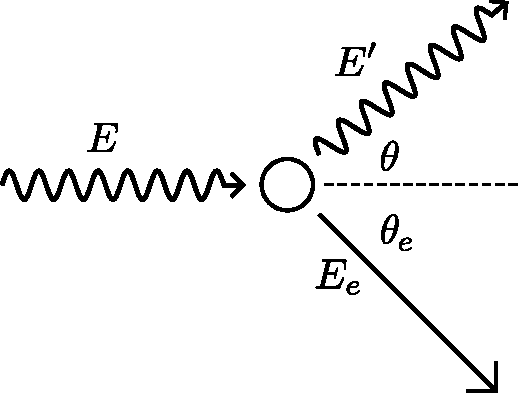
\includegraphics[width = 0.4\colwidth]{compton_diagram.pdf}
        \caption{A diagram representing Rayleigh scattering.}
      \end{figure}

    \end{multicols}

    \begin{center}
      \textbf{3. Rayleigh Scattering}
      \begin{itemize}
        \item Photon interacts coherently with atom, resulting in photon scattering with no energy loss.
      \end{itemize}
      \vspace{-1\baselineskip}
      \begin{figure}
        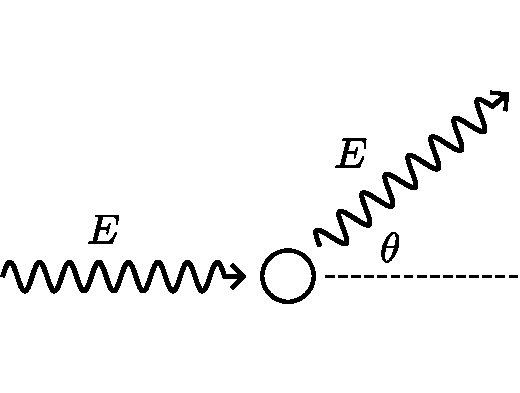
\includegraphics[width = 0.4\colwidth]{rayleigh_diagram.pdf}
        \caption{A diagram representing Compton scattering.}
      \end{figure}
    \end{center}
    \vspace{-\baselineskip}
  \end{block}

  \begin{center}
    \textbf{Implementation}
  \end{center}

  For coherent and incoherent scattering, the methodology of \cite{lund2018implementation} was adapted for use in MIDSX, neglecting Doppler energy broadening and the production of secondary particles. For the photoelectric effect, the photon is terminated and all energy is deposited at the location of interaction.

  \begin{block}{Validation}

    To validate the accuracy of MIDSX, simulations were performed and compared to reference data (PENELOPE, EGSrnc, Geant4, and MCNP) obtained by the American Association of Physicists in Medicine Task Group Report 195 (TG-195) \cite{sechopoulos_monte_2015}.

    % \begin{figure}
    %   \centering
    %   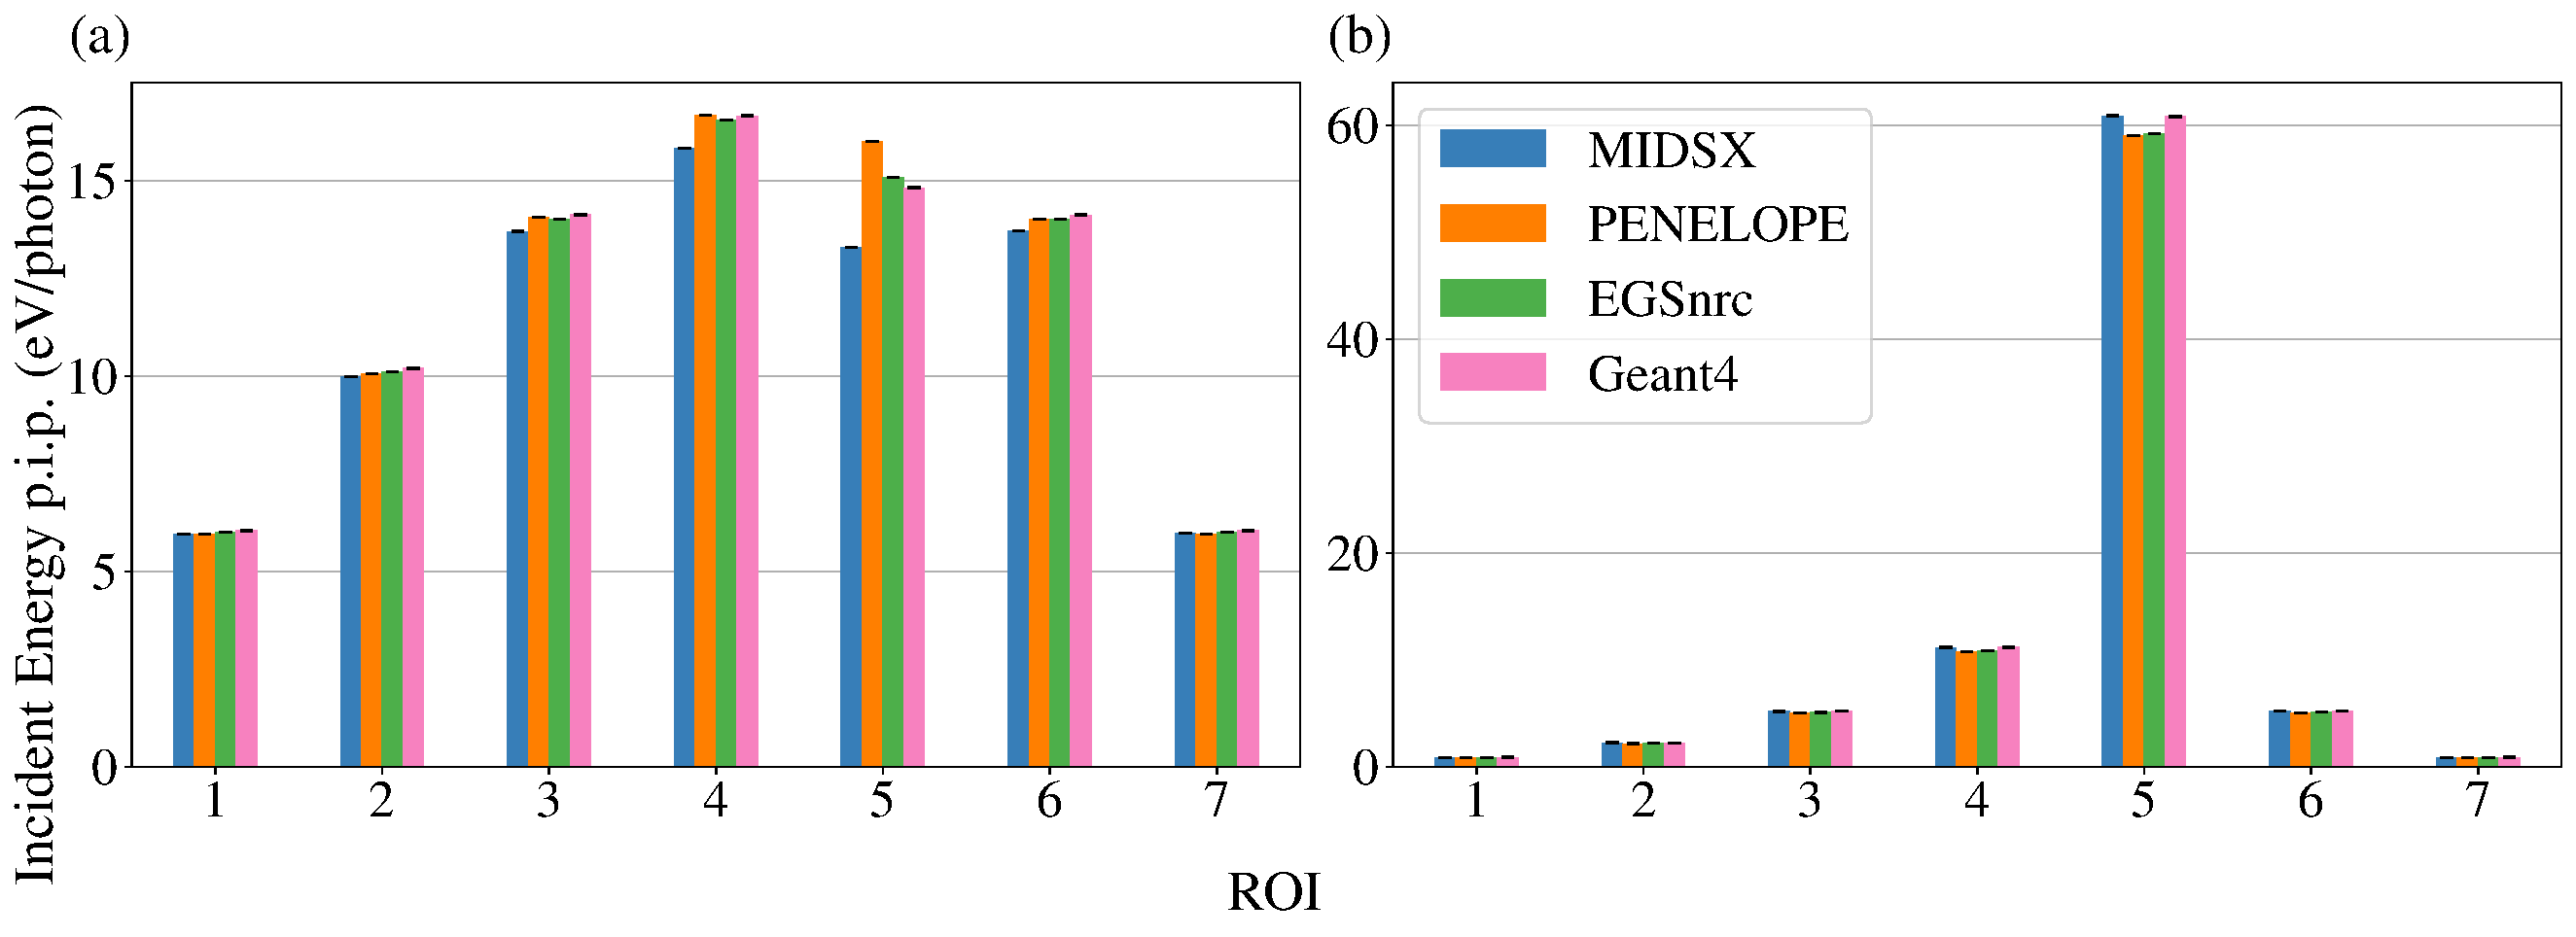
\includegraphics[width = \colwidth]{ROI_0_deg__pencil_paper_ready_wo_mutiple.pdf}
    %   \caption{The energy per initial photon (p.i.p.) (eV/photon) of photons incident upon each region of interest (ROI) for the $0^\circ$, pencil beam, 56.4 keV simulation as described by Case 2. The incident energy was determined separately for photons that underwent (a) a single incoherent scatter and (b) a single coherent scatter.}
    %   \label{fig:ROIPGraph}
    % \end{figure}
  \end{block}

\end{column}

\separatorcolumn

\begin{column}{\colwidth}

  \vspace{-2\baselineskip}  
\begin{figure}[htbp]
  \hspace*{8mm} % Adjust the 5mm as needed to shift to the right
  \centering
  \zz{radiography_body_dep_poster_ready}
  \caption{The energy deposited per initial photon (p.i.p.) (eV/photon) in the simulated tissue for the full-field simulation as described by Case 2. The simulation was performed at 56.4 keV and 120 kVp at $0^\circ$, with the 120 kVp spectrum provided by TG-195.}
  \label{fig:BDGraph}
\end{figure}


    \begin{figure}
      \centering
    % 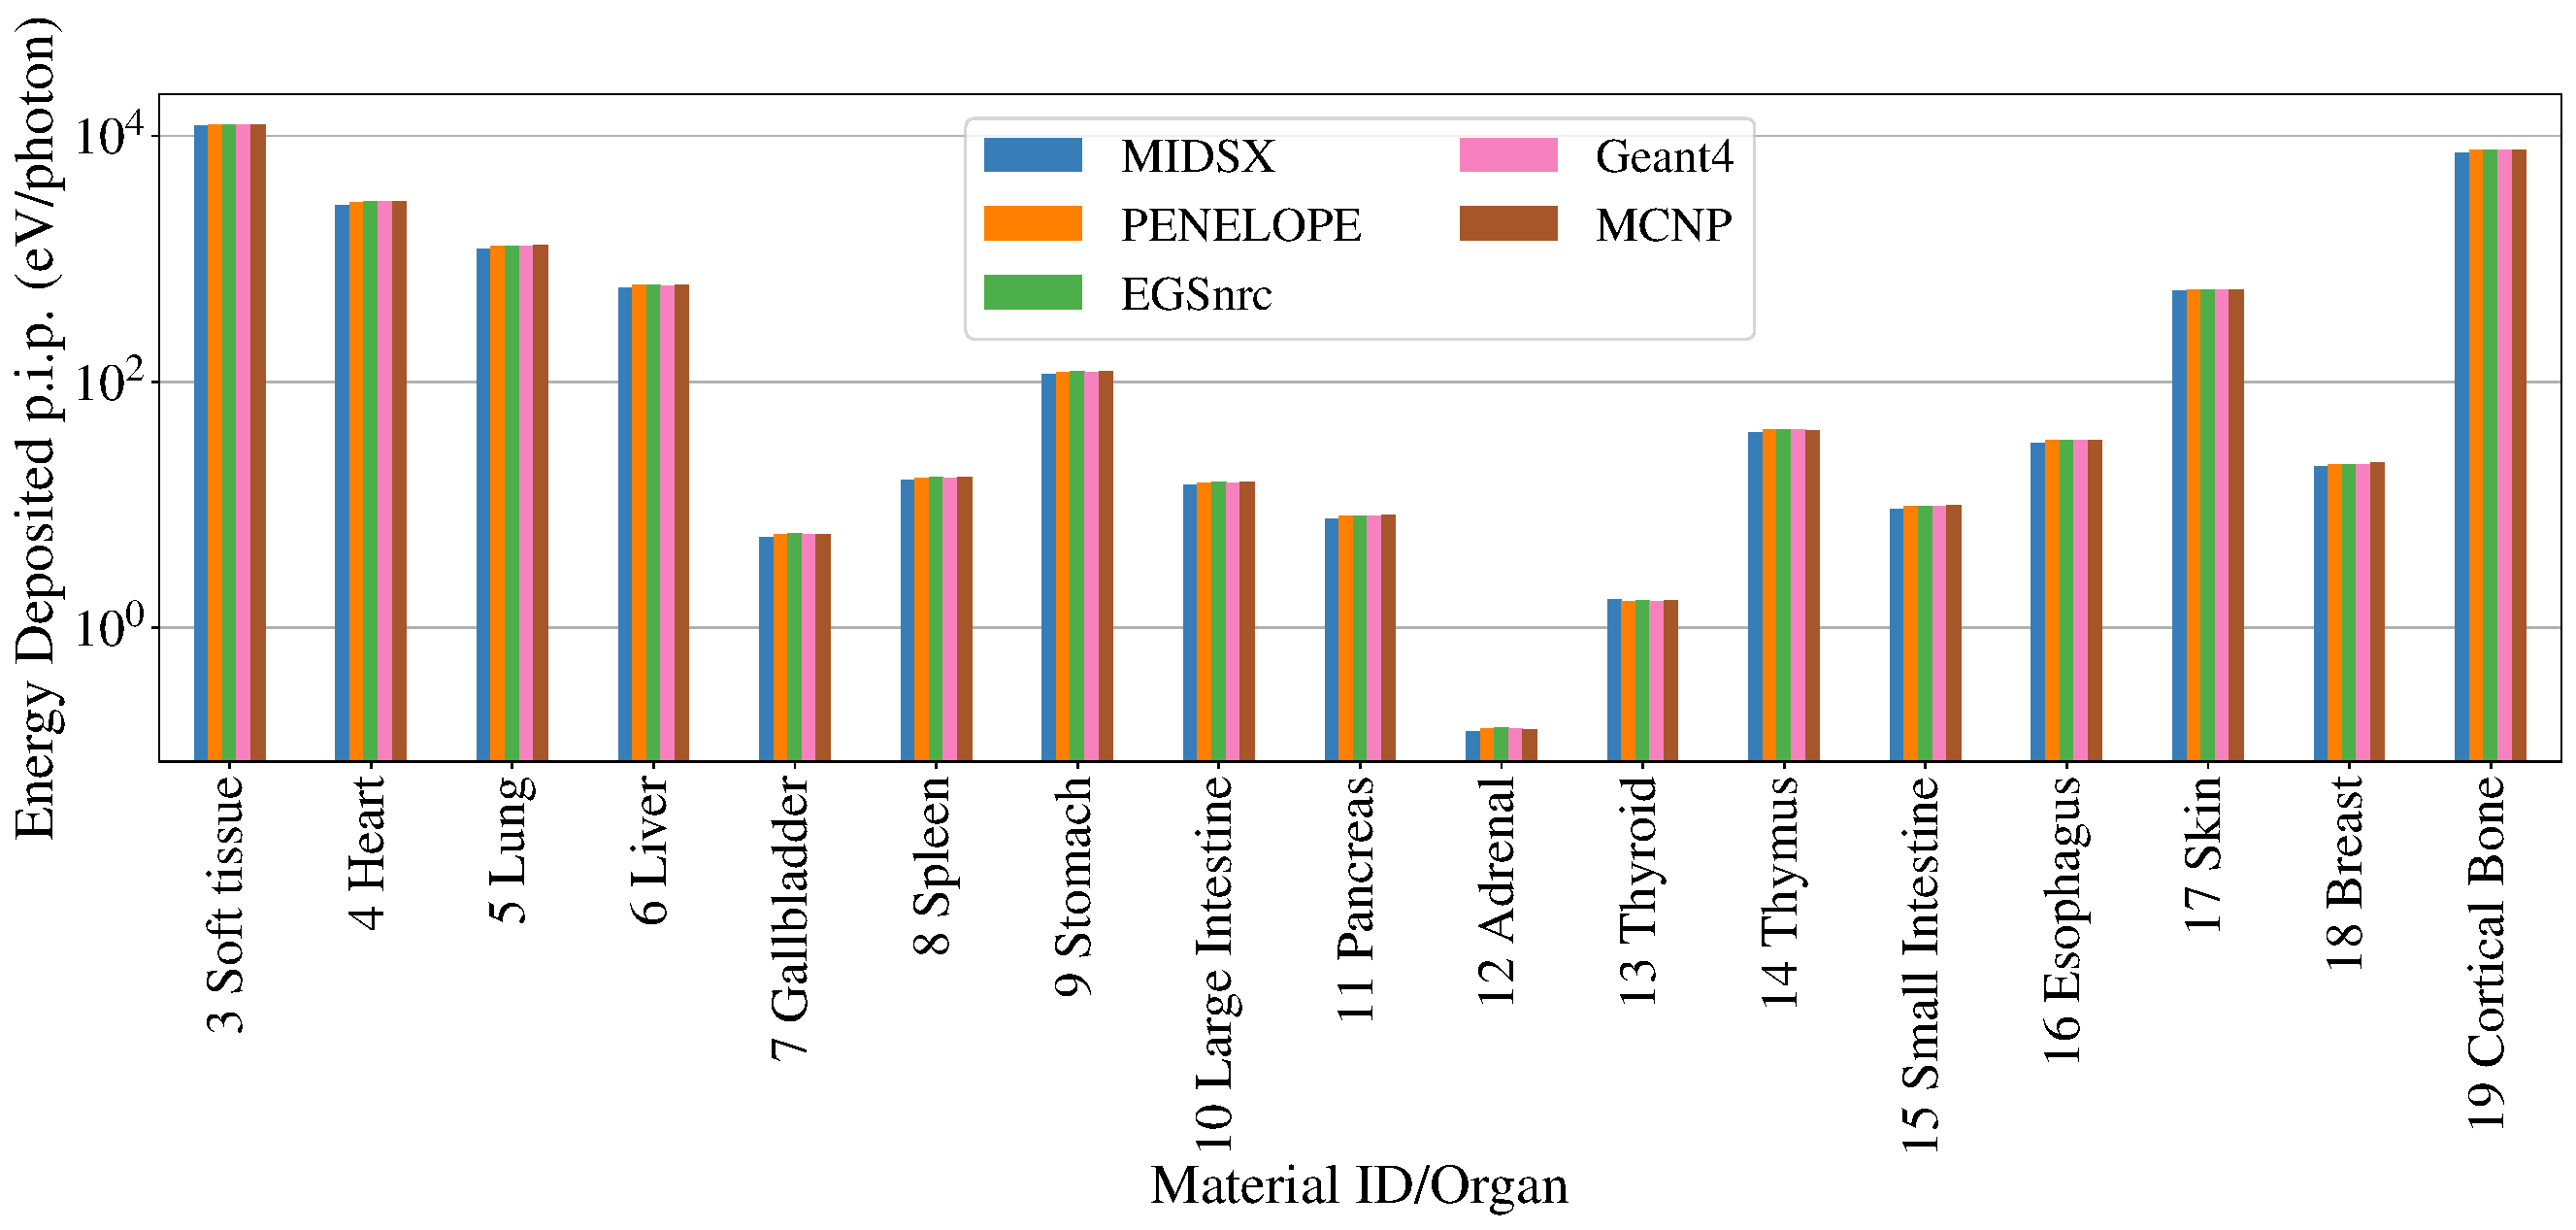
\includegraphics[width= \colwidth]{CT_120_0_big_font.pdf}
    \zz{CT_120_0_big_font}
    \caption{The energy deposited per initial photon (p.i.p.) (eV/photon) in the organs composing a voxelized human phantom for the $0^\circ$, 120 kVp simulation as described by Case 5.}
    \label{fig:CTGraph}
    \end{figure}
  

  \begin{block}{Discussion}

  \begin{itemize}
      \item MIDSX demonstrates varied but reasonable agreement with TG-195 reference code systems, with excellent agreement in Case 1 and 2.
      \item For Case 5, all organ energy depositions were lower than reference codes, except for the thyroid. The max mean percent error observed was 6.3\%.
      % \item Orientation verification through root mean square percent error (RMSPE) analysis suggests correct phantom orientation in CT simulations, pointing to other errors in MIDSX that require further investigation.
      \item Future work will focus on investigating the implementation of scattering events, cross-section data initialization, and interpolation errors in MIDSX.
  \end{itemize}
    
  \end{block}
  \vspace{-1\baselineskip}
  \begin{block}{References}

    % \nocite{*}
    \vspace{-0.5\baselineskip}
    \footnotesize{\bibliographystyle{unsrt}\bibliography{poster}}

  \end{block}

\end{column}

\separatorcolumn
\end{columns}
\end{frame}

\end{document}
